\section{Methodology}\label{sec:methodology}

This section presents the methodology adopted in this study. Figure~\ref{fig:workflow} provides an overview of the flow from data acquisition to final model evaluation. It preserves the practical sequence of the IJCNN precursor---input data, technical indicators, feature selection, optimization, model fitting, and evaluation---while inserting the temporal controls and the two validation objectives required by the expanded benchmark.

\begin{figure}[htbp]
\centering
\resizebox{0.96\linewidth}{!}{%
\begin{tikzpicture}[
  node distance=0.72cm and 0.62cm,
  every node/.style={draw=black!80,rounded corners=2.5pt,align=center,minimum height=0.88cm,text width=2.75cm,font=\footnotesize},
  process/.style={fill=black!5}, protocol/.style={fill=black!12,text width=3.15cm},
  outcome/.style={fill=black!18,text width=4.10cm}, arrow/.style={-{Stealth[length=2.0mm]},thick}
]
  \node[process] (data) {\textbf{Input data}\\WIN five-minute futures\\$N=15{,}057$ bars};
  \node[process, right=of data] (indicators) {\textbf{Technical indicators}\\66 price, moving-average, volatility, volume, and trading descriptors};
  \node[process, right=of indicators] (selection) {\textbf{Feature selection}\\Information Gain\\seven retained features};
  \node[process, below=1.05cm of indicators] (split) {\textbf{Temporal data partition}\\chronological 60/20/20\\train, validation, locked test};
  \node[process, below=of split] (search) {\textbf{Equal-budget optimizer search}\\RS, GA, PSO, DE, and GWO\\$N_{\mathrm{eval}}=1{,}000$ per seed};
  \node[protocol, below left=0.92cm and 0.25cm of search] (mcc) {\textbf{Protocol A: MCC/$F_1$ fitness}\\$0.60\,\mathrm{MCC}_{\mathrm{val}}+0.40\,F_{1,\mathrm{val}}$};
  \node[protocol, below right=0.92cm and 0.25cm of search] (accuracy) {\textbf{Protocol B: accuracy fitness}\\$0.40\,\mathrm{Acc}_{\mathrm{train}}+0.60\,\mathrm{Acc}_{\mathrm{val}}$};
  \coordinate (protocolmid) at ($(mcc.south)!0.5!(accuracy.south)$);
  \node[outcome, below=1.00cm of protocolmid] (test) {\textbf{Model fitting and locked evaluation}\\RF, SVM, MLP, and 1D-CNN; common seeds 1--3\\held-out accuracy, MCC, $F_1$, and intraday economic evaluation};
  \draw[arrow] (data) -- (indicators); \draw[arrow] (indicators) -- (selection);
  \draw[arrow] (selection.south) |- (split.east); \draw[arrow] (split) -- (search);
  \draw[arrow] (search) -- (mcc); \draw[arrow] (search) -- (accuracy);
  \draw[arrow] (mcc.south) |- (test.west); \draw[arrow] (accuracy.south) |- (test.east);
\end{tikzpicture}%
}
\caption{Overview of the proposed methodology. The new benchmark preserves the precursor workflow while enforcing a chronological split, equal optimizer budget, and two separated validation objectives.}
\label{fig:workflow}
\end{figure}

\subsection{Input Data}
\label{sec:data}

The data were obtained from the BovDB resources \cite{cardoso2022bovdb,souza2024dataset}. The analyzed subset contains 15,057 clean five-minute records of the WIN contract from January to June 2024. WIN is referenced to the Ibovespa index and was selected because its liquidity and frequent intraday movement make it suitable for short-horizon computational prediction. The binary target indicates the next-bar direction: 0 for downtrend and 1 for uptrend.

The records remain in chronological order. The first 9,034 observations are used for training, the subsequent 3,011 observations for validation, and the final 3,012 observations for locked testing. No random shuffling is applied. Figure~\ref{fig:partition} makes this separation explicit; the test observations are unavailable during both feature and hyperparameter selection.

\begin{figure}[htbp]
\centering
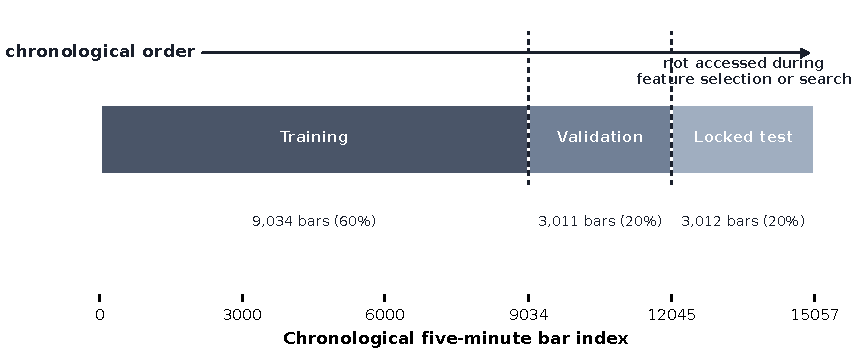
\includegraphics[width=0.93\linewidth]{figures/ijcnn_style_partition.pdf}
\caption{Chronological data partition used in every experiment. Training, validation, and locked test segments occupy consecutive periods of the WIN five-minute series.}
\label{fig:partition}
\end{figure}

\subsection{Generation of Technical Analysis Indicators}
\label{sec:indicators}

Technical indicators were derived from open, high, low, close, trade volume, and transaction-frequency information. Simple Moving Average (SMA), Exponential Moving Average (EMA), and dispersion measures were computed over short windows (3, 5, 7, and 9 periods) to retain sensitivity to intraday changes. For example, the difference between the seven- and three-period SMA is
\begin{equation}
\mathrm{SMA}_{7-3}=\mathrm{SMA}_{7}-\mathrm{SMA}_{3}.
\end{equation}
The raw and derived variables were normalized before model fitting. Together, the construction procedure produces 66 descriptors, including moving-average differences and normalized counterparts.

\subsection{Feature Selection Method}
\label{sec:featureselection}

The indicator pool is reduced using Information Gain, as in the precursor. This filter selects attributes that most reduce uncertainty regarding the next-bar direction and avoids repeating highly redundant descriptors in each search evaluation \cite{lei2012feature,kumar2014feature}. Seven features are retained: EMA$_{5-3}$, normalized EMA$_{5-3}$, EMA$_{7-3}$, normalized EMA$_{7-3}$, normalized SMA$_9$, EMA$_{9-3}$, and normalized EMA$_7$. The same reduced representation is used by all model and optimizer combinations.

\subsection{Optimizer Configuration and Validation Objectives}
\label{sec:optimizerconfiguration}

Five optimizers are evaluated: RS, GA, PSO, DE, and GWO. Each optimizer receives 1,000 candidate evaluations for each model and seed. Population-based methods use populations of ten candidates, corresponding to 100 generations or iterations; RS samples 1,000 feasible configurations. GA uses tournament selection, crossover, and mutation; PSO uses inertia plus cognitive and social terms; DE uses the best/1/bin strategy; and GWO updates candidate positions from its leading agents.

Two validation objectives are evaluated. Protocol A uses the compound metric
\begin{equation}
f_{\mathrm{MCC/F1}}(\boldsymbol{\theta})=0.60\,\mathrm{MCC}_{\mathrm{val}}(\boldsymbol{\theta})+0.40\,F_{1,\mathrm{val}}(\boldsymbol{\theta}),
\end{equation}
whereas Protocol B uses
\begin{equation}
f_{\mathrm{Acc}}(\boldsymbol{\theta})=0.40\,\mathrm{Accuracy}_{\mathrm{train}}(\boldsymbol{\theta})+0.60\,\mathrm{Accuracy}_{\mathrm{val}}(\boldsymbol{\theta}).
\end{equation}
After candidate selection, the selected configuration is refit on training plus validation data and evaluated once on the locked test block.
